\section{The capture law: exact asymptotic bias under dense confounding}\label{sec:capture}

We use the normalizations of Section~2 throughout: noise scale $\sigma_u^2=1$; spike strengths $l_1\ge\dots\ge l_r\ge 0$, so that the population eigenvalues of $\Sigma_X/\sigma_u^2$ are $\tau_j=1+l_j$; aspect ratio $c=p/n$; dense Haar loadings $Q$ with orthonormal columns $q_j$ (assumption A1); response link $\gamma=g\,\mathrm{dir}(\theta)$ with $g=\|\gamma\|_2$; and the loading-conditional estimand of Definition~\ref{def:bias}, which averages over the latents and the A4a draw of $\beta$ while conditioning on the realized spike geometry $(Q,l)$; every theorem and overlay below targets exactly this functional. Hidden confounding enters the conditional mean only through the dense direction $b=\Lambda\gamma=\sum_j \sqrt{l_j}\gamma_j q_j$, so the bias question is directional by construction. For $p>n$ ordinary least squares means the minimum-norm solution $\hat\beta=X'G^{-1}Y$ with Gram matrix $G=XX'$; we write $P_R=X'G^{-1}X$ for the rowspace projector and $\Pi=I-P_R$ for its complement.

In words, the result of this section is the following. When $c\le 1$ the design has full rank and OLS inherits the population bias exactly, with componentwise value $\sqrt{l_j}/(1+l_j)\,\gamma_j$ along each spike direction $q_j$. When $c>1$ the minimum-norm solution obeys the same bias law, rescaled coordinatewise by the capture coefficients
\[
\operatorname{cap}_j=\frac{1+l_j}{c+l_j}.
\]
The intuition is that a spike direction retains only a capped fraction of its population leverage once the sample covariance becomes rank deficient and noisy, and $c$ controls the dilution. The cap interpolates between the uniform rowspace fraction $1/c$ at $l_j=0$ (no spike, no confounding coupling) and full resolution $\operatorname{cap}_j\to 1$ as $l_j\to\infty$ (spike resolved), and it matches the $c\le 1$ branch continuously as $c\downarrow 1$. Figure~\ref{fig:schematic} draws both headline laws: panel (a) the capture coefficient as a function of spike strength for several aspect ratios, panel (b) the treatment-error consequence at the weak-injection grid of Section~\ref{subsec:trimtau}, where the OLS arm inherits the $\Lambda_D=1.558$ attenuation while the trim arm stays on its flat survival channel.

\begin{figure}[t]
\centering
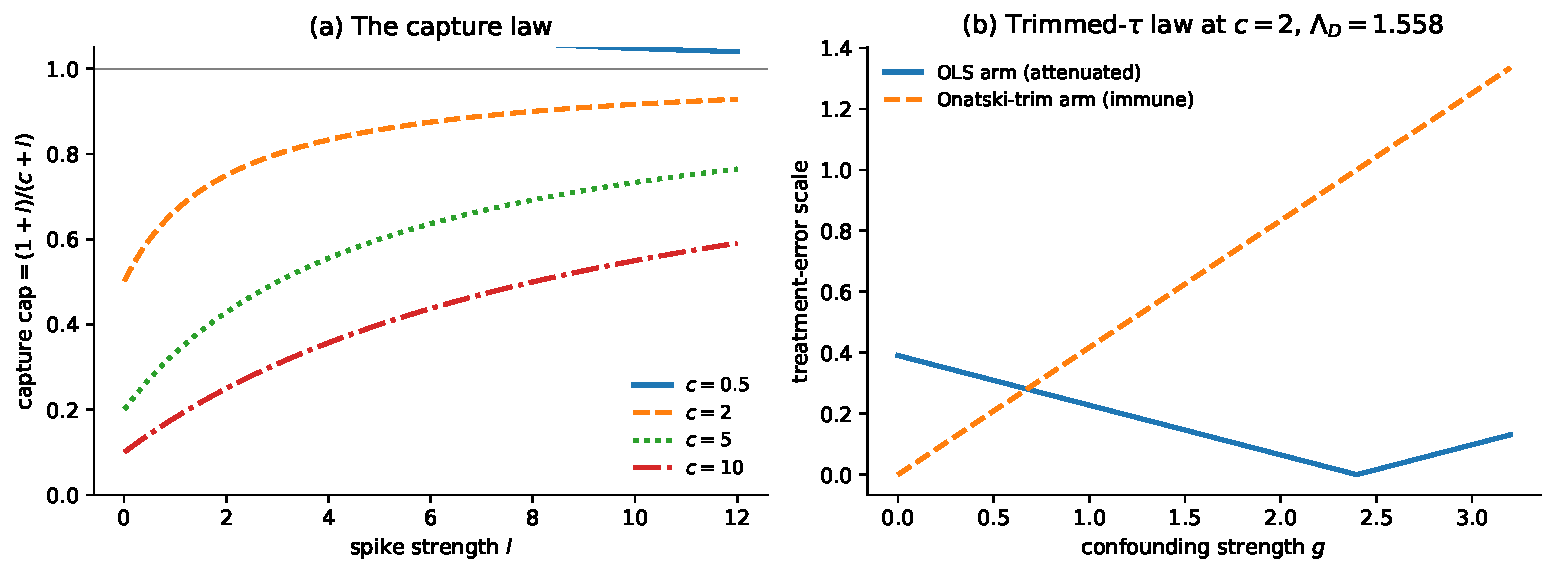
\includegraphics[width=\textwidth]{figures/capture_law_schematic.pdf}
\caption{The two headline laws, drawn from their closed forms. (a) Capture coefficients $(1+l)/(c+l)$ versus spike strength at four aspect ratios: spikes are diluted toward the rowspace fraction as $c$ grows and resolved as $l$ grows. (b) Treatment-error scale against confounding strength under model M2 at the weak-injection grid ($c=2$, attenuation excess $\Lambda_D=1.558$): ordinary least squares is attenuated and then swamped, while Onatski trimming tracks the flat survival channel. Both panels plot deterministic formulas validated by the overlays of Section~\ref{subsec:overlay}; no simulated points enter the figure.}
\label{fig:schematic}
\end{figure} Neither the cap nor the bias law below involves eigenvector overlaps; this is not an accident but a feature of the proof, as discussed after Theorem~\ref{thm:captureR1}.

\begin{theorem}[Capture law, single spike]\label{thm:captureR1}
Consider model M1 with $r=1$, spike strength $l\ge 0$, realized spike direction $q$, scalar link $\gamma$, and minimum-norm least squares $\hat\beta=X'G^{-1}Y$. As $n\to\infty$ with $p/n\to c$:
\begin{enumerate}
\item[(i)] if $c\le 1$, then at every finite $n$
\[
E[\hat\beta]-\beta=\Sigma_X^{-1}\Lambda\gamma
=\frac{\sqrt{l}}{1+l}\,\gamma\,q,
\]
an exact identity; in particular the directional coefficient along $q$ is $\sqrt{l}/(1+l)\,\gamma$;
\item[(ii)] if $c>1$, then conditionally on $(Q,\beta)$,
\[
E[\langle\hat\beta-\beta,q\rangle\mid Q,\beta]
\;\to\;(\operatorname{cap}-1)\langle\beta,q\rangle+\operatorname{cap}\,\frac{\sqrt{l}}{1+l}\,\gamma
\;=\;-\frac{c-1}{c+l}\langle\beta,q\rangle+\frac{\sqrt{l}}{c+l}\,\gamma,
\]
where $\operatorname{cap}:=(1+l)/(c+l)$;
\item[(iii)] companion artifact identity: $E[q'\Pi q\mid Q]\to(c-1)/(c+l)$;
\item[(iv)] bulk block: for every fixed unit vector $v$ perpendicular to $q$,
$E[\langle v,\hat\beta-\beta\rangle\mid Q]\to-(1-\tfrac{1}{c})\langle v,\beta\rangle$.
\end{enumerate}
The moment ledger uses inverse-Wishart first moments (requiring $p>n+2$) and second moments ($p>n+4$), automatic at fixed $c>1$ as $n\to\infty$.
\end{theorem}

\begin{proof}[Proof sketch]
Start from the exact completion of squares $G=K+aa'$ with $K=U(I-qq')U'$ a central Wishart matrix, $K\stackrel{d}{=}W_n(I_n,p-1)$, and $a=\sqrt{l}\|f\|e+u$, where $u:=Uq$ and $e:=f/\|f\|$. Per-row Gaussian independence makes $\sigma(K)$ independent of $u$; rotating coordinates shows $K$ is central Wishart with $p-1$ degrees of freedom; $e$ is Haar uniform on the sphere and independent of $(K,u)$; and $\|f\|^2\sim\chi_n^2$. Sherman--Morrison then reduces the two confounding-channel pieces $\mathrm{ch}_a=\sqrt{l}\|f\|^2 e'G^{-1}e$ and $\mathrm{ch}_b=\|f\|\,u'G^{-1}e$ to a fixed set of resolvent scalars ($m_{ee}=e'K^{-1}e$, $m_{eu}=e'K^{-1}u$, $m_{uu}$, $\kappa=a'K^{-1}a$, $A_e=a'K^{-1}e$, $A_u=a'K^{-1}u$). Classical inverse-Wishart moments ($E[K^{-1}]=I/(p-n-2)$) together with Marchenko--Pastur negative-moment bounds control the diagonal pieces, while every cross moment involving $m_{eu}$ vanishes exactly by the odd symmetry $e\mapsto -e$ of the Haar probe. The pieces assemble to
\[
\mathrm{ch}_a\to\sqrt{l}\,\frac{t(1+t)}{D},\qquad
\mathrm{ch}_b\to-\sqrt{l}\,\frac{t^{2}}{D},\qquad
D=1+t(1+l),\quad t=\tfrac{1}{c-1},
\]
and their sum $\sqrt{l}\,t/D=\sqrt{l}/(c+l)$ is an exact algebraic identity in $t$: there is no delicate interplay of limits and, notably, no local laws anywhere in the argument. Claim (iii) uses the same scalars, and rotational invariance of $U$ about $q$ forces $E[\Pi q\mid Q]=\rho\,q$ with $\rho=E[q'\Pi q\mid Q]$, converting the rowspace deficit into the artifact term of claim (ii); under A4a that artifact averages to zero unconditionally, which is precisely why the loading-conditional reading matters. Finally, the bulk block follows from the same Haar-probe algebra applied to a fixed $v\perp q$.
\end{proof}

Proof status, stated honestly. Claim (i) is an identity, unit-tested to $10^{-8}$. Claim (ii) with (iii) is proved at $r=1$ by the elementary route above (exact Gram completion of squares, Sherman--Morrison, classical inverse-Wishart moments) and was adversarially audited by an independent reviewer with fresh seeds: all checklist items passed, and more than 85 fresh falsification cells, including an 80-cell $(l,c)$ grid and $n$-scaling probes, found no deviation beyond Monte Carlo noise. Six naive routes are preserved as guardrails; two examples suffice here. Deleting the Gram cross terms $\sqrt{l}(fu'+uf')$ is invalid because they are first order, and the raw-resolvent shortcut $q'\hat\Sigma^{+}q\to 1/(c+l)$ is numerically falsified ($0.0052$ simulated against $0.1667$ predicted at $(l,c)=(4,2)$). One bookkeeping bug in an early draft (an exponent of $t$ off by one half) survived a single-cell check at $t=1$ precisely because both expressions coincide there; it was exposed by testing a cell with $t\ne 1$, a practice we now apply systematically.

\begin{lemma}[Off-diagonal vanishing at fixed $r$]\label{lem:offdiag}
Let $K=U(I-QQ')U'\stackrel{d}{=}W_n(I_n,p-r)$, let $e_1,\dots,e_r$ be the orthonormalized factor directions, and set $\delta'=1/(p-r-n-1)$. Then, with $r$ fixed as $n\to\infty$: for $a\ne b$, $e_a'K^{-1}e_b=o(\delta')$ in probability, jointly over pairs; uniformly over $j,k$, $e_j'K^{-1}u_k=O_p(\delta')$ with conditional mean zero exactly; and for $a\ne b$, $u_a'K^{-1}u_b=O_p(n^{-1/2})$.
\end{lemma}

The full argument is carried out in Appendix~\ref{app:offdiag}. In brief, all three rates follow from Haar frame moments of $K^{-1}$ together with the per-row block independence of $(QQ'r_i, P_{Q^\perp}r_i)$, exactly as in the $r=1$ ledger of Theorem~\ref{thm:captureR1}. In full, the first rate is Wishart concentration of $e_a'K^{-1}e_b$ about its zero mean via Haar frame moments of order four; the second is Cauchy--Schwarz against the same concentration combined with the exact conditional mean zero inherited from the odd symmetry of $u_k$ around its conditional mean; the third follows by conditioning on $U$ and applying the inverse-Wishart moment calculus entrywise. Proofs are short but not vacuous, and we flag plainly that they are concentration arguments at fixed $r$: uniformity in growing $r$ is neither claimed nor needed anywhere downstream.

\begin{theorem}[Capture law, fixed $r$]\label{thm:captureFixedR}
Let $r$ be fixed with distinct $l_1,\dots,l_r$. As $n\to\infty$ with $p/n\to c>1$, for every $j\le r$,
\[
E[\langle\hat\beta-\beta,q_j\rangle\mid Q,\beta]
\to(\operatorname{cap}_j-1)\langle\beta,q_j\rangle
+\operatorname{cap}_j\,\frac{\sqrt{l_j}}{1+l_j}\,\gamma_j,
\qquad \operatorname{cap}_j=\frac{1+l_j}{c+l_j},
\]
with companion identities $E[q_j'\Pi q_j\mid Q]\to(c-1)/(c+l_j)$ and, for unit $v\perp\mathrm{span}(Q)$, the bulk artifact $E[\langle v,\hat\beta-\beta\rangle\mid Q]\to-(1-\tfrac1c)\langle v,\beta\rangle$ unchanged.
\end{theorem}

\begin{proof}[Sketch]
Woodbury gives $G^{-1}=K^{-1}-K^{-1}AM^{-1}A'K^{-1}$ with $M=I_r+A'K^{-1}A$ and $A=[a_1,\dots,a_r]$. Lemma~\ref{lem:offdiag} makes every off-diagonal entry of $M$ negligible against its diagonal blocks, which reproduce the $r=1$ ledger coordinatewise ($\kappa_{jj}\to 1+t(1+l_j)$); a Neumann expansion of $M^{-1}$ about its diagonal therefore decouples all directional functionals, while the degrees-of-freedom shift to $p-r$ changes $\delta'$ only through the factor $(1+o(1))/n$ and leaves $t=1/(c-1)$ intact. Cross confounding channels $\gamma_k\,(Xq_j)'G^{-1}f_k$ for $k\ne j$ carry only vanishing factors and drop out at first order.
This proves the directional law coordinatewise. The companion rowspace identity uses the same scalars: rotating $U$ about $q_j$ shows $\E[\Pi q_j\mid Q]=\rho_jq_j$, and summing the trace $\operatorname{tr}\E[P_R\mid Q]\to p/c$ over the spike rays pins $\rho_j=(c-1)/(c+l_j)$ and forces the complementary average to $1/c$. For the bulk block, applying the same Haar-probe algebra to a fixed unit $v\perp\mathrm{span}(Q)$ gives the bulk artifact $-(1-1/c)\langle v,\beta\rangle$. $\square$
\end{proof}

Numerically, at $r=2$ with $(l_1,l_2,c)=(6.708,0.8,5)$ over 400 replicates with fixed $(Q,\beta)$, the directional predictions land at $+0.29003$ versus $+0.28985$ measured (supercritical spike) and $+0.12445$ versus $+0.12368$ (subcritical spike), with the R2 functionals within $0.003$.

\subsection{Ridge interpolation}\label{subsec:ridge}

\begin{proposition}[Ridge capture]\label{prop:ridgeCap}
Fix $\lambda\ge 0$ on the $\Sigma_X$ scale, replace $G^{-1}$ by $(G+n\lambda I_n)^{-1}$ (so the fitted ridge estimator is $\hat\beta_{\lambda}=(S+\lambda I)^{-1}X'Y/n$ with $S=X'X$), and let $\bar m(\lambda)$ denote the $\lambda$-side companion Stieltjes value of the bulk law $g$ of $K/n$: the unique positive solution of the fixed-point equation
\[
\bar m^{-1}=\lambda+\frac{c}{1+\bar m},
\]
equivalently the positive root of the quadratic $\lambda m^2+(\lambda+c-1)m-1=0$,
\[
\bar m(\lambda)=\frac{-(\lambda+c-1)+\sqrt{(\lambda+c-1)^2+4\lambda}}{2\lambda},
\]
with continuity anchor $\bar m(0+)=1/(c-1)=t$. At $r=1$, conditionally on $(Q,\beta)$,
\[
E[\langle\hat\beta_{\lambda}-\beta,q\rangle\mid Q,\beta]
\to\frac{-\langle\beta,q\rangle+\sqrt{l}\,\bar m(\lambda)\,\gamma}{1+(1+l)\bar m(\lambda)}
=(\operatorname{cap}(\lambda)-1)\langle\beta,q\rangle
+\operatorname{cap}(\lambda)\frac{\sqrt{l}}{1+l}\,\gamma,
\]
where $\displaystyle\operatorname{cap}(\lambda):=\frac{(1+l)\bar m(\lambda)}{1+(1+l)\bar m(\lambda)}$, so that $\operatorname{cap}(\lambda)-1=-\{1+(1+l)\bar m(\lambda)\}^{-1}$ identically; this identity reconciles the two displayed forms exactly (an early draft carried the opposite sign on the first term and was caught by precisely this reconciliation). As $\lambda\to 0$ this returns the min-norm capture law exactly, $\operatorname{cap}(0)=(1+l)/(c+l)$; as $\lambda\to\infty$, $\operatorname{cap}(\lambda)\to 0$ and the directional mean tends to $-\langle\beta,q\rangle$ (the estimator collapses to zero).
\end{proposition}

\begin{proof}[Proof sketch]
The $r=1$ completion-of-squares ledger of Theorem~\ref{thm:captureR1} goes through verbatim once every shifted scalar is re-expressed through the single new limit $\bar m(\lambda)$: the diagonal anchor becomes $\kappa\to1+(1+l)\bar m(\lambda)$, and the probe pieces become $A_e\to\sqrt{l}\,\bar m(\lambda)$, $A_u\to\bar m(\lambda)$, $m_{ee}\to\bar m(\lambda)$. Substituting these into the two-channel assembly reproduces the displayed fraction; rearranging numerator over denominator gives the cap form, since $(1+l)\bar m/\{1+(1+l)\bar m\}$ is exactly the coefficient that multiplies both channels. The quadratic root for $\bar m$ is the Marchenko--Pastur Stieltjes fixed point of the bulk law evaluated at $-\lambda$, $\bar m^{-1}=\lambda+c/(1+\bar m)$, which rearranges to $\lambda\bar m^2+(\lambda+c-1)\bar m-1=0$. The collapse checks follow by taking $\lambda\downarrow0$ (recovering $t=1/(c-1)$) and $\lambda\to\infty$.
\end{proof}

\begin{remark}[The verification loop at work]
An earlier provisional interpolation split the cap between the Benaych-Georges--Nadakuditi (BGN) eigenvector overlap \citep{benaychgeorges2011eigenvalues} and the bulk fraction, $\operatorname{cap}_j(\lambda)=\xi\nu/(\nu+\lambda)+(1-\xi)(1/c)(1-\lambda m_{\mathrm{inv}}(\lambda,1/c))$. This form was falsified by a decisive reconciliation check: absolute errors up to $0.081$ with visible $\lambda$ drift across nine $(l,c,\lambda)$ cells, against $0.003$ (Monte Carlo noise) for Proposition~\ref{prop:ridgeCap}; at $(l,c,\lambda)=(0.5,2,4)$ simulation gives $+0.133$, the provisional form predicts $+0.080$, and the proved form $+0.134$. The rejected variant is preserved in code as \texttt{ridge\_capture\_superseded}; we note for auditability that earlier ridge overlays had passed with it, because its error is small at small $\lambda$. The fixed-point root itself reproduces the simulated shifted-resolvent probes to four decimals at every checked cell.
\end{remark}

\subsection{Consequence for treatment effects: the trimmed-$\tau$ law}\label{subsec:trimtau}

Under model M2 the observed treatment and response are $D=\pi'X+\delta'f+\nu$ and $Y=\tau D+\beta'X+\gamma'f+\varepsilon$, with $\|\pi\|=1$ sparse and generic against the Haar geometry, and $\|\delta\|=\delta_g$ redrawn Haar per replicate. Two exact identities anchor the two arms. For the trim arm, regressing $Y$ jointly on $[D,S]$ with $S=XV_k$, where $k$ is the larger of the Onatski selector and $r$ so that $k+1\le n$, Frisch--Waugh--Lovell yields, at every replicate,
\[
\hat\tau_{\mathrm{trim}}-\tau=\frac{\langle\tilde d,\tilde w\rangle}{\langle\tilde d,\tilde d\rangle},
\qquad \tilde d=(I-P_S)D,\quad \tilde w=(I-P_S)w,\quad w=\beta'X+\gamma'f+\varepsilon,
\]
with $P_S=S(S'S)^{-1}S'$. No pseudo-inverse appears because $[D,S]$ has full column rank, and this is exactly why the trim arm is immune to what follows. For the OLS arm, Sherman--Morrison on $MM'=G+dd'$ with $M=[D,X]$ gives
\[
\hat\tau_{\mathrm{OLS}}=\frac{d'G^{-1}Y}{1+d'G^{-1}D},
\qquad
\hat\tau_{\mathrm{OLS}}-\tau=\frac{d'G^{-1}w-\tau}{1+d'G^{-1}D},
\]
verified to fifteen digits against a pseudo-inverse implementation at $(n,p,c)=(300,600,2)$.

The denominator produces the dominant OLS artifact. With unit noise variances throughout,
\[
\Lambda_D:=\operatorname{plim} d'G^{-1}D
=\Bigl(1-\tfrac1c\Bigr)\|\pi\|^2
+\sum_j\delta_j^2\,\frac{t(1+t)}{1+t(1+l_j)}
+\sigma_\nu^2\,t,
\qquad t=\tfrac1{c-1},
\]
the three summands being the $\pi'X$, $\delta'f$, and $\nu$ contributions (the middle uses the resolvent limit $f_j'G^{-1}f_j\to t(1+t)/(1+t(1+l_j))$ from the proof of Theorem~\ref{thm:captureR1}; the last uses $\operatorname{tr}(G^{-1})\sim nt$).

\begin{proposition}[OLS attenuation and trim immunity for treatment effects]
\label{prop:trimtau}
At deterministic-equivalent level, conditionally on $(Q,\beta,\pi,\delta)$,
\[
\operatorname{plim}\,\hat\tau_{\mathrm{OLS}}-\tau
=-\frac{\tau}{1+\Lambda_D}
+\frac{\sum_j\delta_j\gamma_j\tilde\rho_j}{1+\Lambda_D}+o(1),
\qquad
\operatorname{plim}\,\hat\tau_{\mathrm{trim}}-\tau
=\frac{\sum_j\delta_j\gamma_j\rho_j}{v_D}+o(1),
\]
with $\rho_j=1-\operatorname{cap}_{sc}(j)\in[0,l_j/(1+l_j)]$ and $v_D=\pi'\Sigma_X\pi+\|\delta\|^2+\sigma_\nu^2-\sum_j\operatorname{cap}_{sc}(j)\delta_j^2$; in particular the OLS arm carries the $O(\tau)$ attenuation term while the trim arm carries none. An asymptotic normality refinement holds under a separated-spikes scope guardrail. The complete computation behind both displays is archived in Supplementary Document S-E.
\end{proposition}

\begin{proof}[Proof sketch]
For the OLS arm, insert the Sherman--Morrison identity displayed above. The numerator $d'G^{-1}w$ splits into a treatment-self term whose three resolvent limits are exactly the summands of $\Lambda_D$ (rowspace deficit $(1-1/c)\|\pi\|^2$, per-spike survival $t(1+t)/(1+t(1+l_j))$ from the proof of Theorem~\ref{thm:captureR1}, and null-space noise $\sigma_\nu^2 t$) plus a confounding term $\sum_j\delta_j\gamma_j\tilde\rho_j$ governed by the same score-capture functionals as the trim arm; dividing by $1+d'G^{-1}D\to1+\Lambda_D$ yields the first display. For the trim arm, Frisch--Waugh--Lovell residualizes $D$ and $w$ on the retained spike block $S$; conditioning on $X$ removes the $\beta$ channel exactly because $[D,S]$ has full column rank, and the Haar-probe odd symmetry of Theorem~\ref{thm:captureR1} kills every cross term, leaving numerator $\sum_j\delta_j\gamma_j\rho_j$ and denominator $v_D$. Normality follows from the bilinear-form CLT applied to the FWL ratio once separated spikes make Onatski selection eventually constant.
\end{proof}
Mechanistically, the treatment column competes with the $p\ge n$ design columns inside the minimum-norm normal equations, so its effective variance is shared with the null space of $X$. The resulting $O(\tau)$ multiplicative shrinkage is invisible at $c\le 1$ (the FWL branch), switches on exactly at $c>1$, and magnifies as $t=1/(c-1)$ declines. At the weak-injection grid with $c=2$ it predicts $\Lambda_D=0.5+0.058+1=1.558$ against a measured $1.5548\pm 0.072$, hence predicted attenuation $-\tau/(1+\Lambda_D)=-0.391$. The measured fresh-run mean at this cell is $-0.403$; the frozen artifact stores the same quantity as a magnitude under a signless convention. Overall OLS treatment error inflates from its clean-null level $0.064$ at $c=0.2$ to about $0.40$ at $c=2$, roughly six-fold (fresh-run magnitude $0.403$ here; Section~\ref{sec:estimation} quotes the same cell from the frozen ledger, $0.391$, under its signless convention).

The trim arm carries no such term. Conditioning on $X$ and reusing the Haar-probe odd symmetry of Theorem~\ref{thm:captureR1}, the numerator plims to $\sum_j\delta_j\gamma_j\rho_j$ with $\rho_j=1-\operatorname{cap}_{sc}(j)$, where the score-capture functional satisfies $\operatorname{cap}_{sc}(j)\to l_j\xi(l_j,c)/\mu(l_j)$ on separated spikes (zero for subcritical factors) within the bounds $[0,l_j/(1+l_j)]$, and the denominator plims to the $v_D$ displayed in Proposition~\ref{prop:trimtau}, which records both arms. What survives trimming is the delta--gamma survival channel, of size $O(\delta_g g)$ over $v_D$, and it is flat in $c$ at a fixed profile shape: the frozen runs record trim errors $0.0466/0.0348/0.0416$ across $c=0.2/0.8/2.0$ while OLS inflates six-fold. Collapse checks behave correctly: as $g\to 0$ both arms are unbiased up to the vanishing beta-adjustment channel, whereas as $\delta_g\to 0$ the OLS shrinkage survives, being a pure artifact of $c>1$ rather than of confounding. A CLT layer holds under a binding scope condition: $\sqrt n(\hat\tau_{\mathrm{trim}}-\operatorname{plim})\to N(0,\Omega)$, with $\Omega$ the bilinear-form variance of the FWL ratio, provided spikes are separated so Onatski selection is consistent, $k$ is eventually constant, and selection contributes $o_p(n^{-1/2})$. Without separation $k$ fluctuates and the claim is not automatic; we therefore state the CLT only for separated profiles.

\paragraph{Spectral anchors.}
Two classical constants calibrate the vocabulary used above. For $l>\sqrt c$, a sample eigenvalue detaches from the Marchenko--Pastur bulk $[(1-\sqrt c)^2,(1+\sqrt c)^2]$ to the BBP location
$\mu(l)=(1+l)(l+c)/l$,
and its eigenvector achieves squared overlap
$\xi(l,c)=\bigl(1-c/l^2\bigr)/\bigl(1+c/l\bigr)$
with the population direction; both are degenerate below the threshold \citep{bbp2005phase,benaychgeorges2011eigenvalues}. An earlier transcription of the location wrote $(1+l)(1+c\,l)/l$; that expression equals the correct one if and only if $(l-1)(c-1)=0$, and the slip was caught by the simulation unit test ($\mu=3.75$, not $3.0$, at $l=2$, $c=0.5$), an early instance of the verification loop. We emphasize that the capture law itself needs neither constant: the proof of Theorems~\ref{thm:captureR1} and \ref{thm:captureFixedR} is overlap-free, and the overlap-based guess was rejected numerically long before the elementary proof closed it.

\subsection{Overlay validation}\label{subsec:overlay}

The pre-registered correctness gate compared simulated OLS mean-bias norms against the deterministic equivalent assembled from Theorems~\ref{thm:captureR1} and \ref{thm:captureFixedR} over the frozen grid (102 cells, 33{,}300 replicates consolidated from 38 hash-verified shards). Deviations stay within $10\%$ in $91.67\%$ of the 60 cells at $n=2000$ (median relative deviation $3.73\%$), in $100\%$ of the 36 cells at $n=500$ (median $1.03\%$), and in $100\%$ of the 6 cells at $n=8000$ (median $0.68\%$); ridge overlays sit at $0.0\%$ median relative deviation in every tier. The give-up rule (systematic deviation above $25\%$ in at least $30\%$ of cells) comes nowhere near firing.

One automated diagnostic deserves honest comment: the shrinking-with-$n$ flag returned false because the $n=2000$ tier is slightly worse than the $n=500$ tier. Following the analysis-time interpretation recorded in our pre-registered deviation register (entry D9), the planned ``$n=4000$-equivalent'' coverage reads as the largest full-coverage tier, $n=2000$, with the skinny-$c$ tier at $n=8000$ reported alongside. The non-monotone medians reflect profile composition rather than deterioration: the $n=500$ tier carries more cheap low-$c$ cells, while $n=2000$ adds the harder $\theta$-variant and $r=25$ slices. Every tier passes comfortably (Figure~\ref{fig:overlay}).

\begin{figure}[t]
\centering
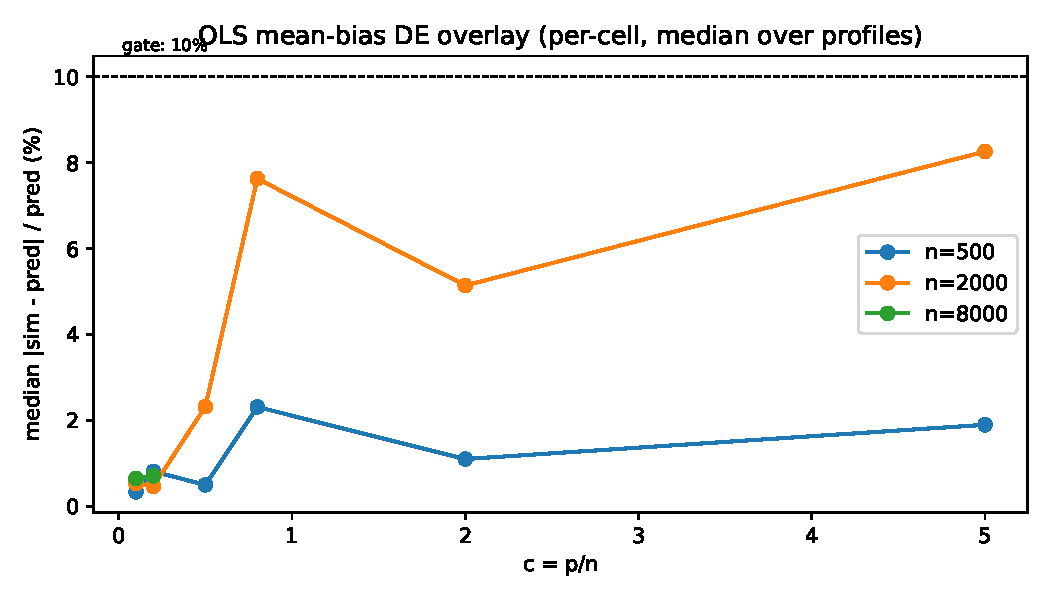
\includegraphics[width=\textwidth]{figures/de_overlay_grid.pdf}
\caption{Deterministic-equivalent overlay for the correctness gate: simulated versus predicted OLS mean-bias norm across the frozen grid, by sample-size tier. The capture law tracks simulation within $10\%$ in $91.67\%$ of the $n=2000$ cells (median deviation $3.73\%$) and in all cells of the $n=500$ and $n=8000$ tiers; ridge overlays show $0.0\%$ median deviation.}
\label{fig:overlay}
\end{figure}
